Rhythm games are a genre of video games that focus on the player’s sense of rhythm and reflexes. They often involve pressing buttons or performing actions in sync with music, creating a unique and engaging experience. The genre has evolved over the years, with various titles introducing innovative gameplay mechanics and input devices. The genre of rhythm games have become popular in both arcades and home consoles, with a wide range of games dedicated to different play styles. The genre has also seen the rise of competitive play, with players striving for high scores and perfect performances. 

\section{Beginning of the genre}
Before one can understand what exactly is behind the term ``rhythm game'', one needs to understand the history and heritage of the genre. The first game to introduce gameplay that somehow resembles part of the mechanics of contemporary rhythm games is \textit{Simon}, created in 1978 by Ralph Baer and Howard Morrison. In this handheld electronic game, the player needs to repeat the sequence in which the buttons light up. The sequence becomes progressively longer, up to the point when a player is unable to repeat it in the right order. There was no background music to speak of, so it cannot be considered a fully-fledged rhythm game, but the action of repeating sequences and patterns is a fundamental part of present-day rhythm games genre.

\begin{figure}[h]
    \centering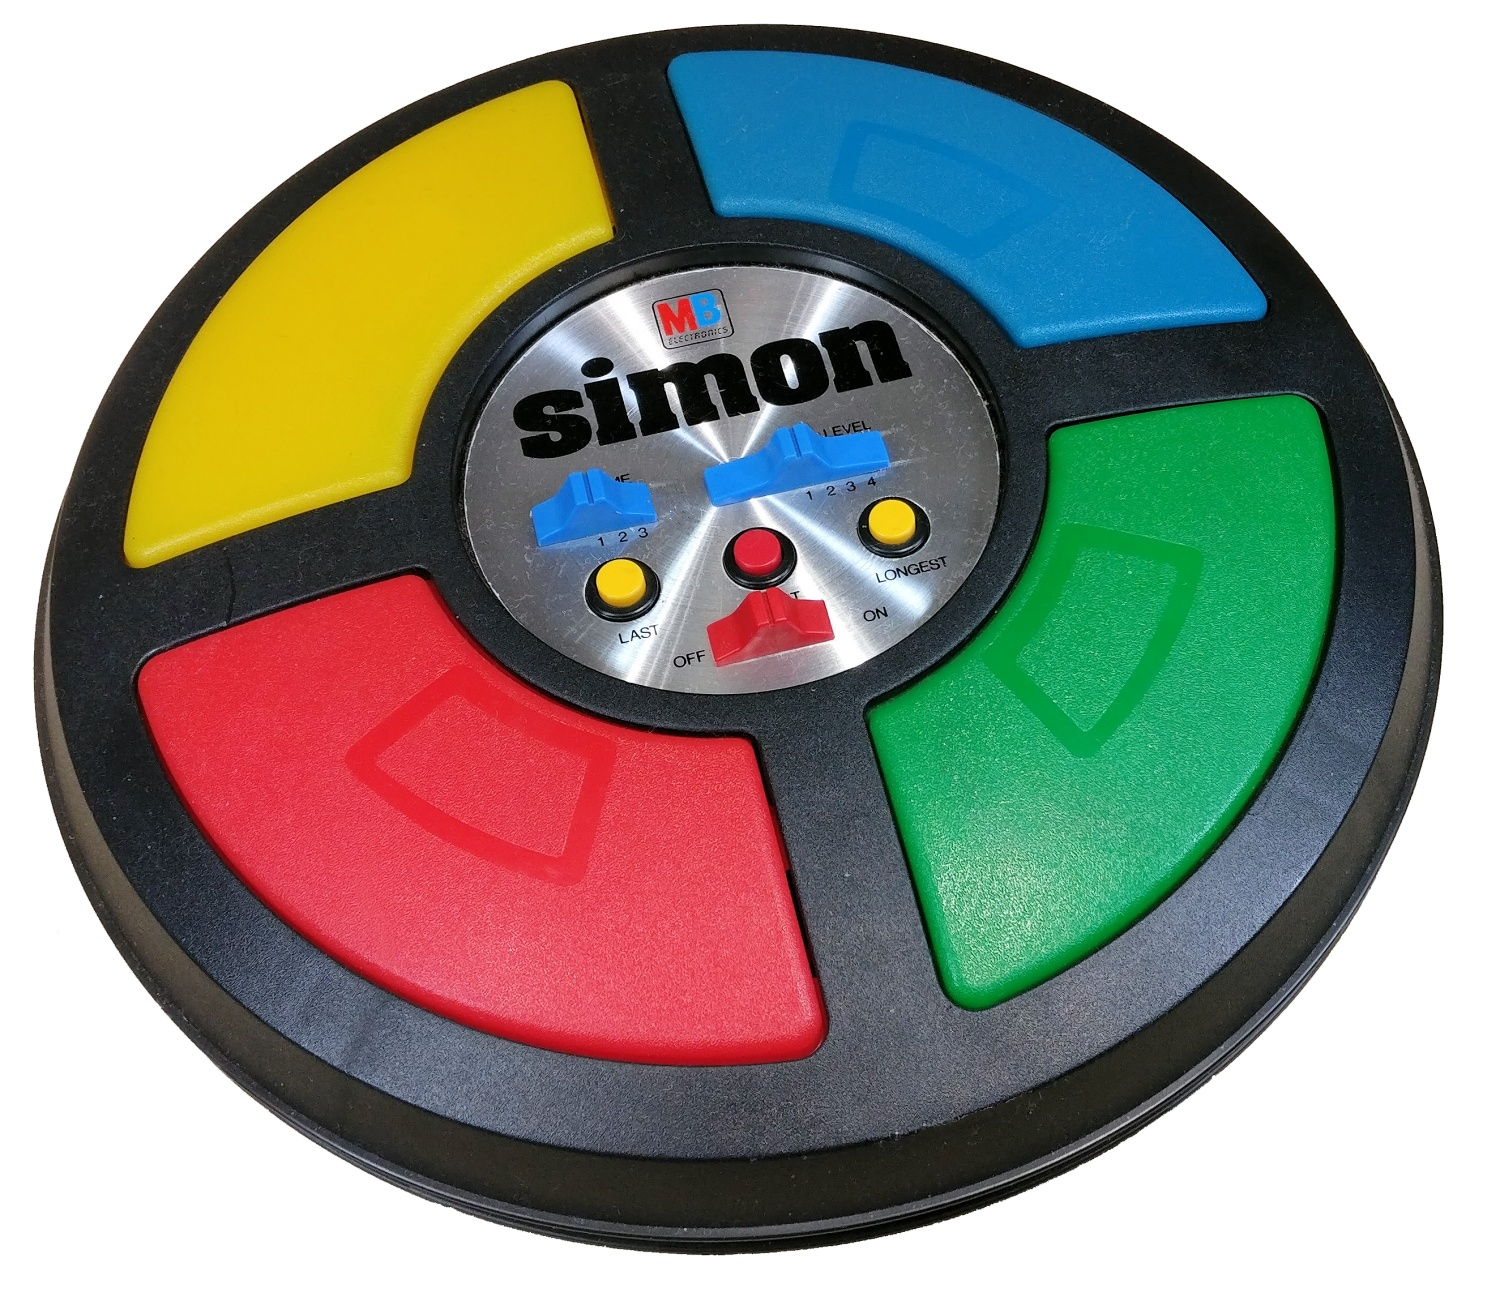
\includegraphics[scale=0.1]{obrazki/simon.jpg}
    \caption{Electronic game \textit{Simon} -- It became a massive worldwide success, becoming a pop culture symbol. The game spawned many different releases and imitators with similar or same basic gameplay. \cite{simongame}}
    \label{fig:simon_game}
\end{figure}

The first rhythm game that can be recognized as such is \textit{PaRappa the Rapper} (1996), published by Sony Computer Entertainment for the PlayStation platform, building its core gameplay around music. Because of its unique art style, good narrative, and catchy soundtrack, the game was well received among players and critics, being listed as one of the best video games ever made several times. \cite{acclaimed_videogames_parappa} This success contributed significantly to the rise in popularity of the genre. In \textit{PaRappa the Rapper}’s gameplay, the player must press correct buttons in response to the rhythm of the currently playing track and symbols that appear on the top of the screen. This mechanic of pressing the corresponding buttons will be further described as ``hit''. The correct sequence is first performed by a teacher, after which PaRappa needs to respond accordingly. Pressing the correct buttons in accordance with the rhythm results in PaRappa rapping. One can observe the resemblance to the aforementioned \textit{Simon} electronic game - PaRappa built upon this mechanic, adding additional visual and auditory feedback, background music and grading system, setting the stage for further developments of this genre. Especially important was the addition of background music synced with other gameplay elements, making it easier to time the hits correctly. The player’s final accuracy is graded from Awful to Cool -- this is currently a standard, expected element of every representative of the genre. The score is affected not only by omitted hits but also by less-than-ideal hits -- the more accurate the hit, the better the rating. As Melanie Fritsch describes in \textit{History of Video Game Music} \cite{MusicMedien}: ``The player had to repeat a sequence of sounds, not only by getting the correct sequence (by hitting the correct buttons), but also by the timing of the sequence. Points were given for correctness as well as for ``style''. For a higher rating, the player had to ``freestyle'', which meant varying from the given sequence but still keeping in time with the song’s rhythm'' (Fritsch 2013: 28).

\begin{figure}[h]
    \centering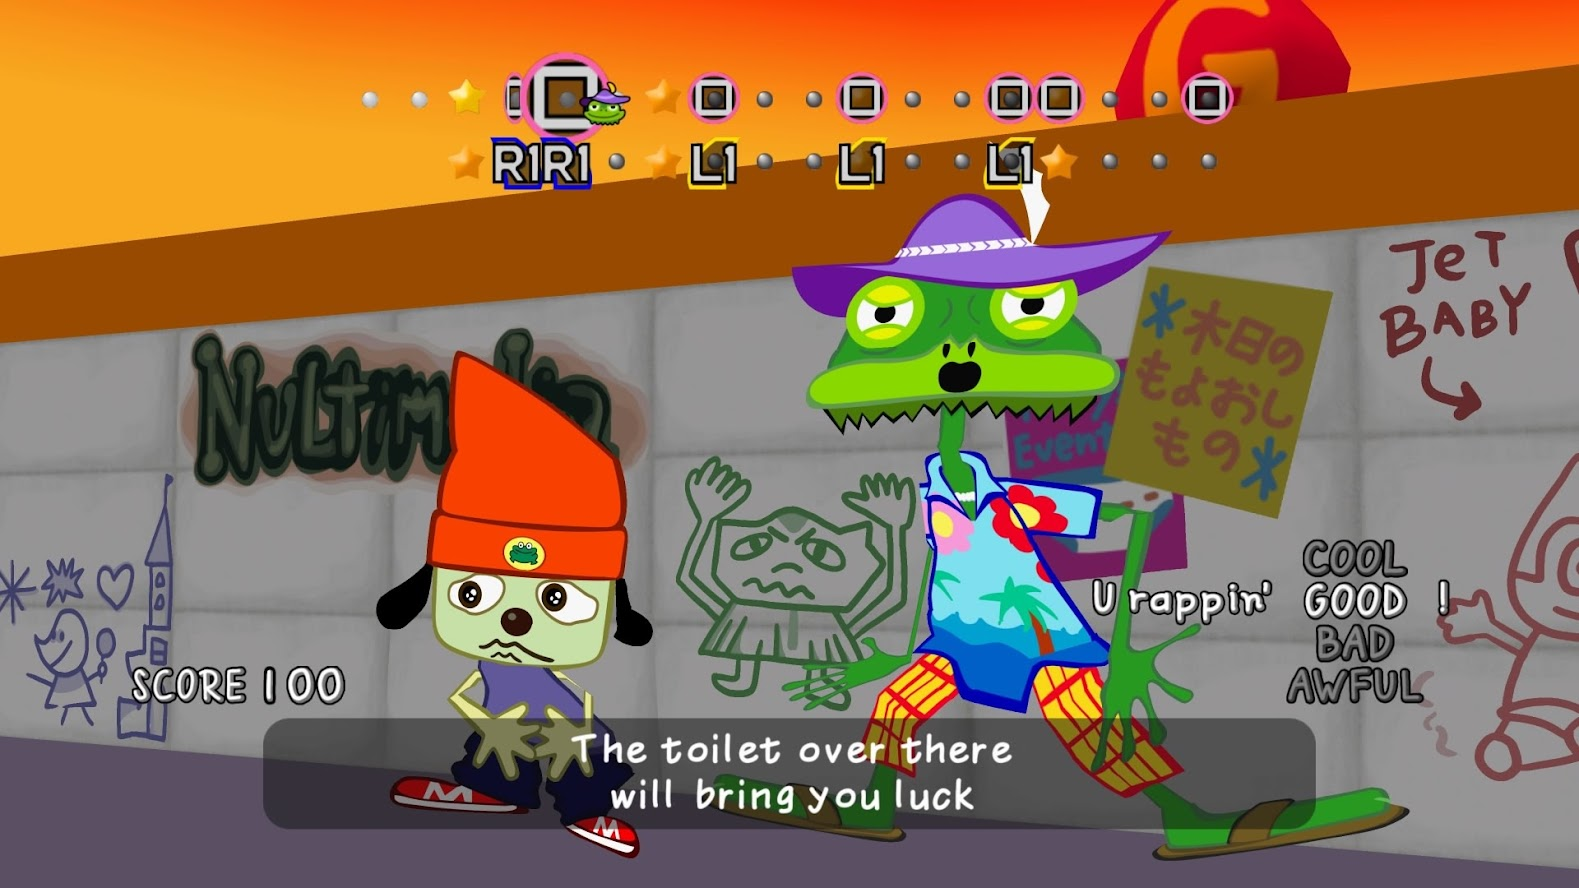
\includegraphics[scale=0.23]{obrazki/parappatherapper.jpg}
    \caption{A frame from \textit{PaRappa the Rapper Remastered} from 2017 showing the input guide at the top of the screen, grading and scoring system. Remastered was used here as an example, but the original had the exact same mechanics back in 1996. \cite{parappatherapper}}
    \label{fig:parappa_the_rapper}
\end{figure}

The release of \textit{beatmania} in 1997 by Konami was another milestone in the development of the rhythm games genre. To enhance the player’s experience with a more immersive input device, the game was introduced to Japanese arcades instead of being released on home platforms. \textit{beatmania}’s arcade cabinet includes a special input device which resembles a DJ console -- it consists of 5 buttons arranged in a piano-like pattern and a round pad that mimics a vinyl record.

\begin{figure}[ht]
    \centering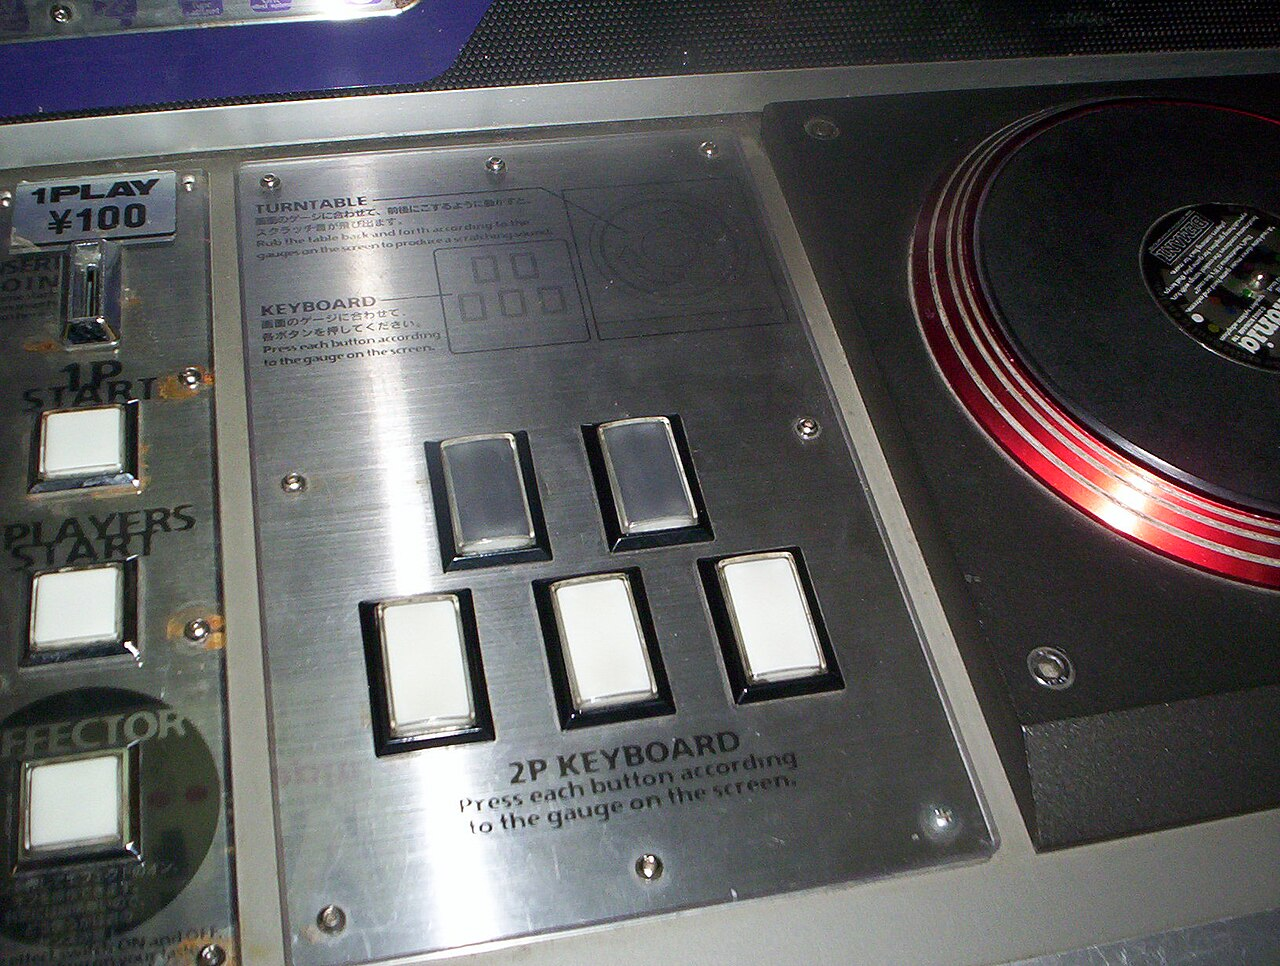
\includegraphics[scale=0.25]{obrazki/beatmaniacontrols.jpg}
    \caption{A controller of 1st \textit{beatmania} arcade release, showing the buttons layout and the turntable. \cite{beatmaniacontrols}}
    \label{fig:beatmania_controls}
\end{figure}

The gameplay is enclosed on a stage that consists of a vertically-scrolling panel with hit-notes on the sides, music video and audience bar in the middle. The player is supposed to press the buttons and turn the turntable in accordance with the notes that are falling from the top to the bottom of the screen, indicating the time to react when they fall down on the judgment line above the illustration of the controller. This is currently known as a vertical scrolling rhythm game -- which \textit{PaRappa the Rapper} could not be considered as such because it showed the input sequences in batches. The game turned out to be a big hit, resulting in Konami putting more effort and resources into Konami’s Games and Music Division. Due to the popularity of \textit{beatmania}, this department changed its name to BEMANI: ``The game was such a huge success that the Games \& Music Division
of the company changed its name to Bemani, which produced and still produces a
long list of spin-offs and sequels'' (Fritsch 2013: 28). \cite{MusicMedien} After experimenting with more concepts of rhythm games, they came up with another big hit, which was \textit{Dance Dance Revolution} (1998) -- a pioneering title in the rhythm game genre. It adapted the basic concept of vertical scrolling rhythm game to a new form of input. The game is controlled through a dance platform, with the player standing in the middle and pressing the buttons with their feet.

The core gameplay is very akin to \textit{beatmania}, sans the turntable. The Vertical Scrolling Rhythm Game (VSRG) formula has been adapted to a new type of play with the player in standing position, dancing to the upcoming rhythm notes. This small change resulted in an experience unlike anything before, as following the patterns became even more natural and dancing became a natural result of playing the game properly. The game became an even bigger success than \textit{beatmania}, achieving worldwide popularity, being an introduction to the rhythm game genre for many players around the world. A major factor in this was definitely the natural connection between its input method and gameplay revolving around dancing.

\begin{figure}[h]
    \centering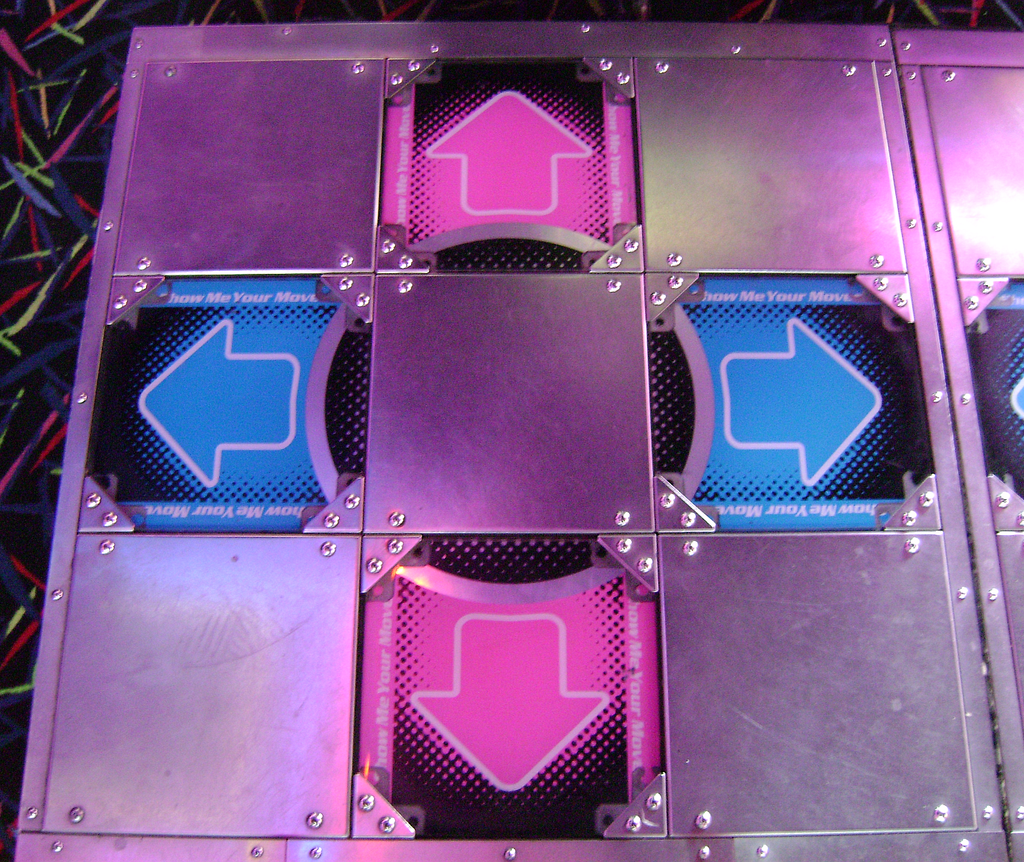
\includegraphics[scale=0.25]{obrazki/ddrplatform.png}
    \caption{A \textit{Dance Dance Revolution} dance platform. \cite{ddrplatform}}
    \label{fig:ddr_platform}
\end{figure}

\begin{figure}[h]
    \centering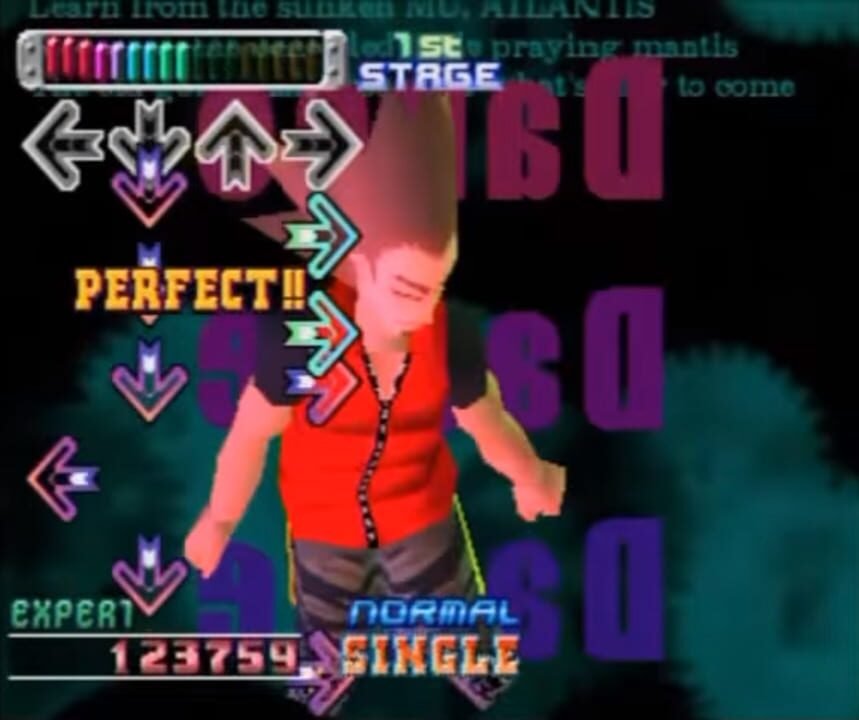
\includegraphics[scale=0.30]{obrazki/ddrgameplay.jpg}
    \caption{\textit{Dance Dance Revolution} gameplay, showing previously described gameplay elements such as health bar and hit notes with matching alignment bar -- taking a form of note outline. Music video is shown playing in the background. \cite{ddrgameplay}}
    \label{fig:ddr_gameplay}
\end{figure}

Taking these games as examples, the core gameplay of all rhythm games is based on performing an action in accordance with the music’s rhythm and displayed pattern. It can be defined that a rhythm game is a medium that puts strong emphasis on a player’s rhythm sense, coordination, and reflexes. Another staple of the medium is often the presence of a custom controller, as demonstrated by \textit{beatmania} and \textit{Dance Dance Revolution}. This stays true to this day -- BEMANI is still publishing new installments of these franchises as of 2024, as well as other rhythm games that incorporate all aforementioned mechanics. An example of another immensely popular series featuring such would be Activision’s \textit{Guitar Hero} series that successfully ported the arcade experience into the living room, bundling the game with the controller starting on the 6th generation of video game consoles. As Andreas Rauscher described in Scoring Play -- Soundtracks and Video Game Genres: ``The user plays the notes shown on the screen with a special game controller reminiscent of a musical toy. Guitar Hero employs a plastic guitar with five buttons simulating the fret and another button used to imitate the strumming.'' (Rauscher 2013: 96) \cite{MusicMedien}.

\begin{figure}[h]
    \centering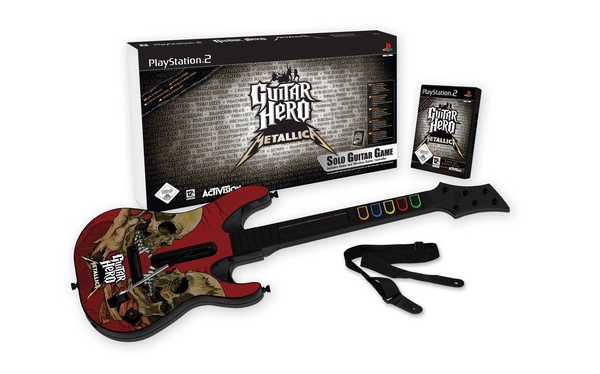
\includegraphics[scale=0.55]{obrazki/gh2bundle.jpg}
    \caption{\textit{Guitar Hero Metallica} PS2 bundle, showing the game disc and plastic guitar controller. \cite{gh2bundle}}
    \label{fig:gh2_bundle}
\end{figure}

The \textit{Guitar Hero} series played crucial part in making rhythm games more popular in the Western regions of the globe, as it featured popular rock and metal songs that attracted new audiences. As Louis-Martin Guay and Dominic Arsenault stated in their chapter of the book \textit{Heavy Metal Generations}: ``Heavy metal and video games share an almost simultaneous birth, with Black Sabbath’s debut album in 1970 and Nolan Bushnell’s Computer Space in 1971. Since the birth of these two subcultures in the early seventies, a growing number of interactions between metal music and video games can be observed'' (Guay and Arsenault 2012: 1). \cite{heavymetal}. In this chapter, authors are describing the relation between this particular music genre and games such as pinballs, arcades, amusement parks and video games. Because musicians saw games and their soundtracks as an opportunity to promote their music and reach new audiences, many bands have started licensing their music to game franchises. Naturally, as music and songs are a crucial part of rhythm games, this genre has been a perfect fit for such collaborations. Furthermore, as \textit{Guitar Hero} revolves around playing guitar, playing favorite heavy metal songs in this game appears as a natural occurrence. Such collaborations have been beneficial for both parties:
\begin{quote}
    ``Just as music or rhythm video games can host heavy metal, so can heavy metal host video games. One of the highest-profile examples of this crossover is the speed power metal band DragonForce, that owes much of its mainstream popularity to the inclusion of their song \textit{‘Through the Fire and Flames’} on Guitar Hero III: Legends of Rock in 2007. Time and again, DragonForce guitarist HermanLi has cited video games as a major influence'' (Guay and Arsenault 2012: 2). \cite{heavymetal}.
\end{quote}
In addition to this mutual benefit between musicians and game developers, the inclusion of songs from real music bands also contributes to the player experience, allowing players to immerse themselves in the game as part of their favorite band. This trope is further reinforced by the Career Mode, the equivalent of the ``story mode'' in other games. In this gamemode, the player is taking a role of a rockstar, making various performances in order to progress as a musician. Such mode provides a sense of progression and achievement, making the game more engaging and rewarding.

\section{Further developments}
Subsequently, rhythm games were released to both arcades and other platforms, such as home and handheld consoles or PCs. In order to relocate the experience of arcade booths into the home, input devices of arcade games were adapted into home versions of dedicated controllers. For example, an open-source project \textit{StepMania}, which is both a PC game and game engine at the same time, was developed with the purpose of replicating the \textit{Dance Dance Revolution} experience at home. It can be played with keyboard or dance pads matching the pattern of \textit{Dance Dance Revolution}, or alternatively following \textit{Pump It Up!} (Andamiro) controls -- a dance game with 4 buttons placed diagonally and one extra button in the middle.

\begin{figure}[h]
    \centering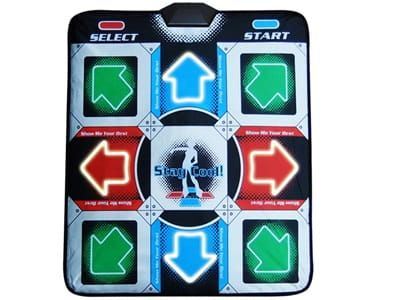
\includegraphics[scale=0.62]{obrazki/ddrsoftpad.jpg}
    \caption{A soft dance-pad which can be used to play both \textit{Dance Dance Revolution} and \textit{Pump it Up!} at home. It can be plugged into a PC or a console. \cite{ddrsoftpad}}
    \label{fig:ddr_softpad}
\end{figure}

In the present day, there are many popular PC games that do not require any dedicated controllers or input devices, making it easier to enter the genre with basic gaming setup. Games such as \textit{StepMania}, \textit{osu!} or \textit{DJMAX} have online scoreboards and online multiplayer modes that bring players together and create lively communities, making the competitive nature a natural part of their gameplay and purpose for players.

\begin{figure}[h]
    \centering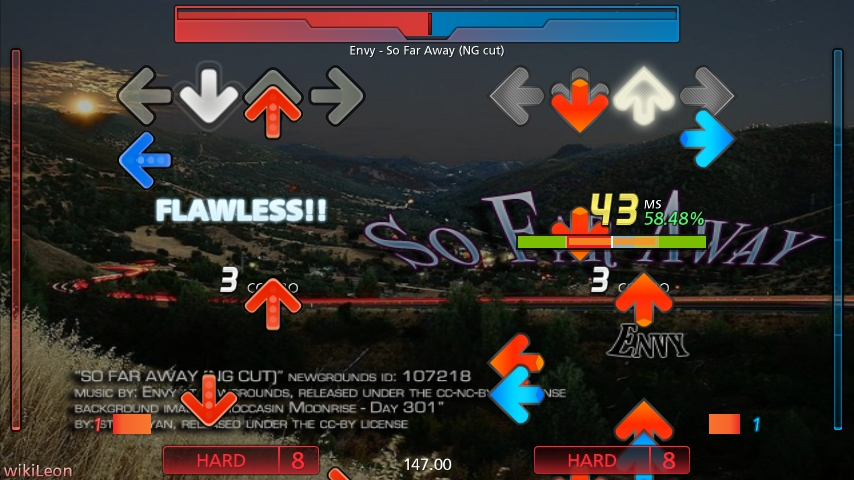
\includegraphics[scale=0.4]{obrazki/sm5multi.jpg}
    \caption{\textit{StepMania} gameplay screenshot, showing Multiplayer Mode where 2 players are competing with each other for better score. \cite{sm5multi}}
    \label{fig:sm5_multi}
\end{figure}

\begin{figure}[h]
    \centering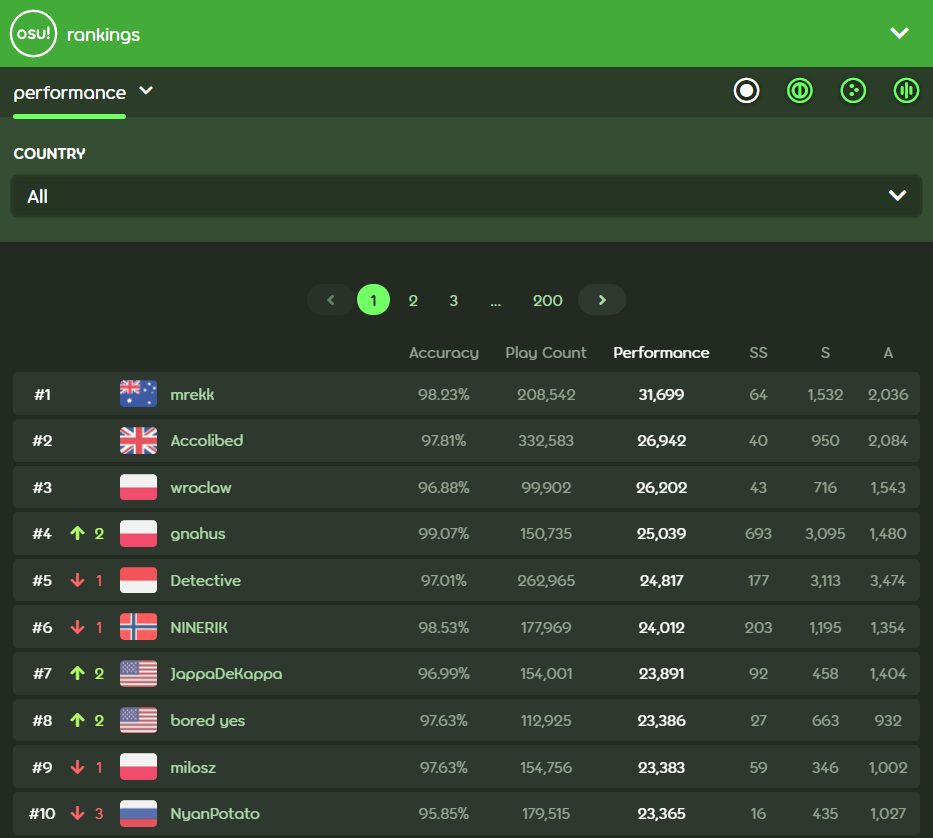
\includegraphics[scale=0.405]{obrazki/osuleaderboards.png}
    \caption{\textit{osu!} online leaderboards as of Jan 2025, showing top players performance from around the world. \cite{osuleaderboards}}
    \label{fig:osu_leaderboards}
\end{figure}
 
On the other hand, there are many arcade games that have unique controllers of various forms. One such arcade game that is worth mentioning is \textit{WACCA}, developed and published by Marvelous, which was created in collaboration with HARDCORE TANO*C and released in 2020. The game’s user interface is enclosed in a circle, surrounded by a circular, segmented ring panel on the screen edges. The notes appear on the center screen, approaching the player through the ring panels. Because of its fun form somehow resembling a washing machine drum, this game stands out from other rhythm game arcades, as it’s financially unviable to port to a home console or PC due to this control scheme and gameplay.

\begin{figure}[h]
    \centering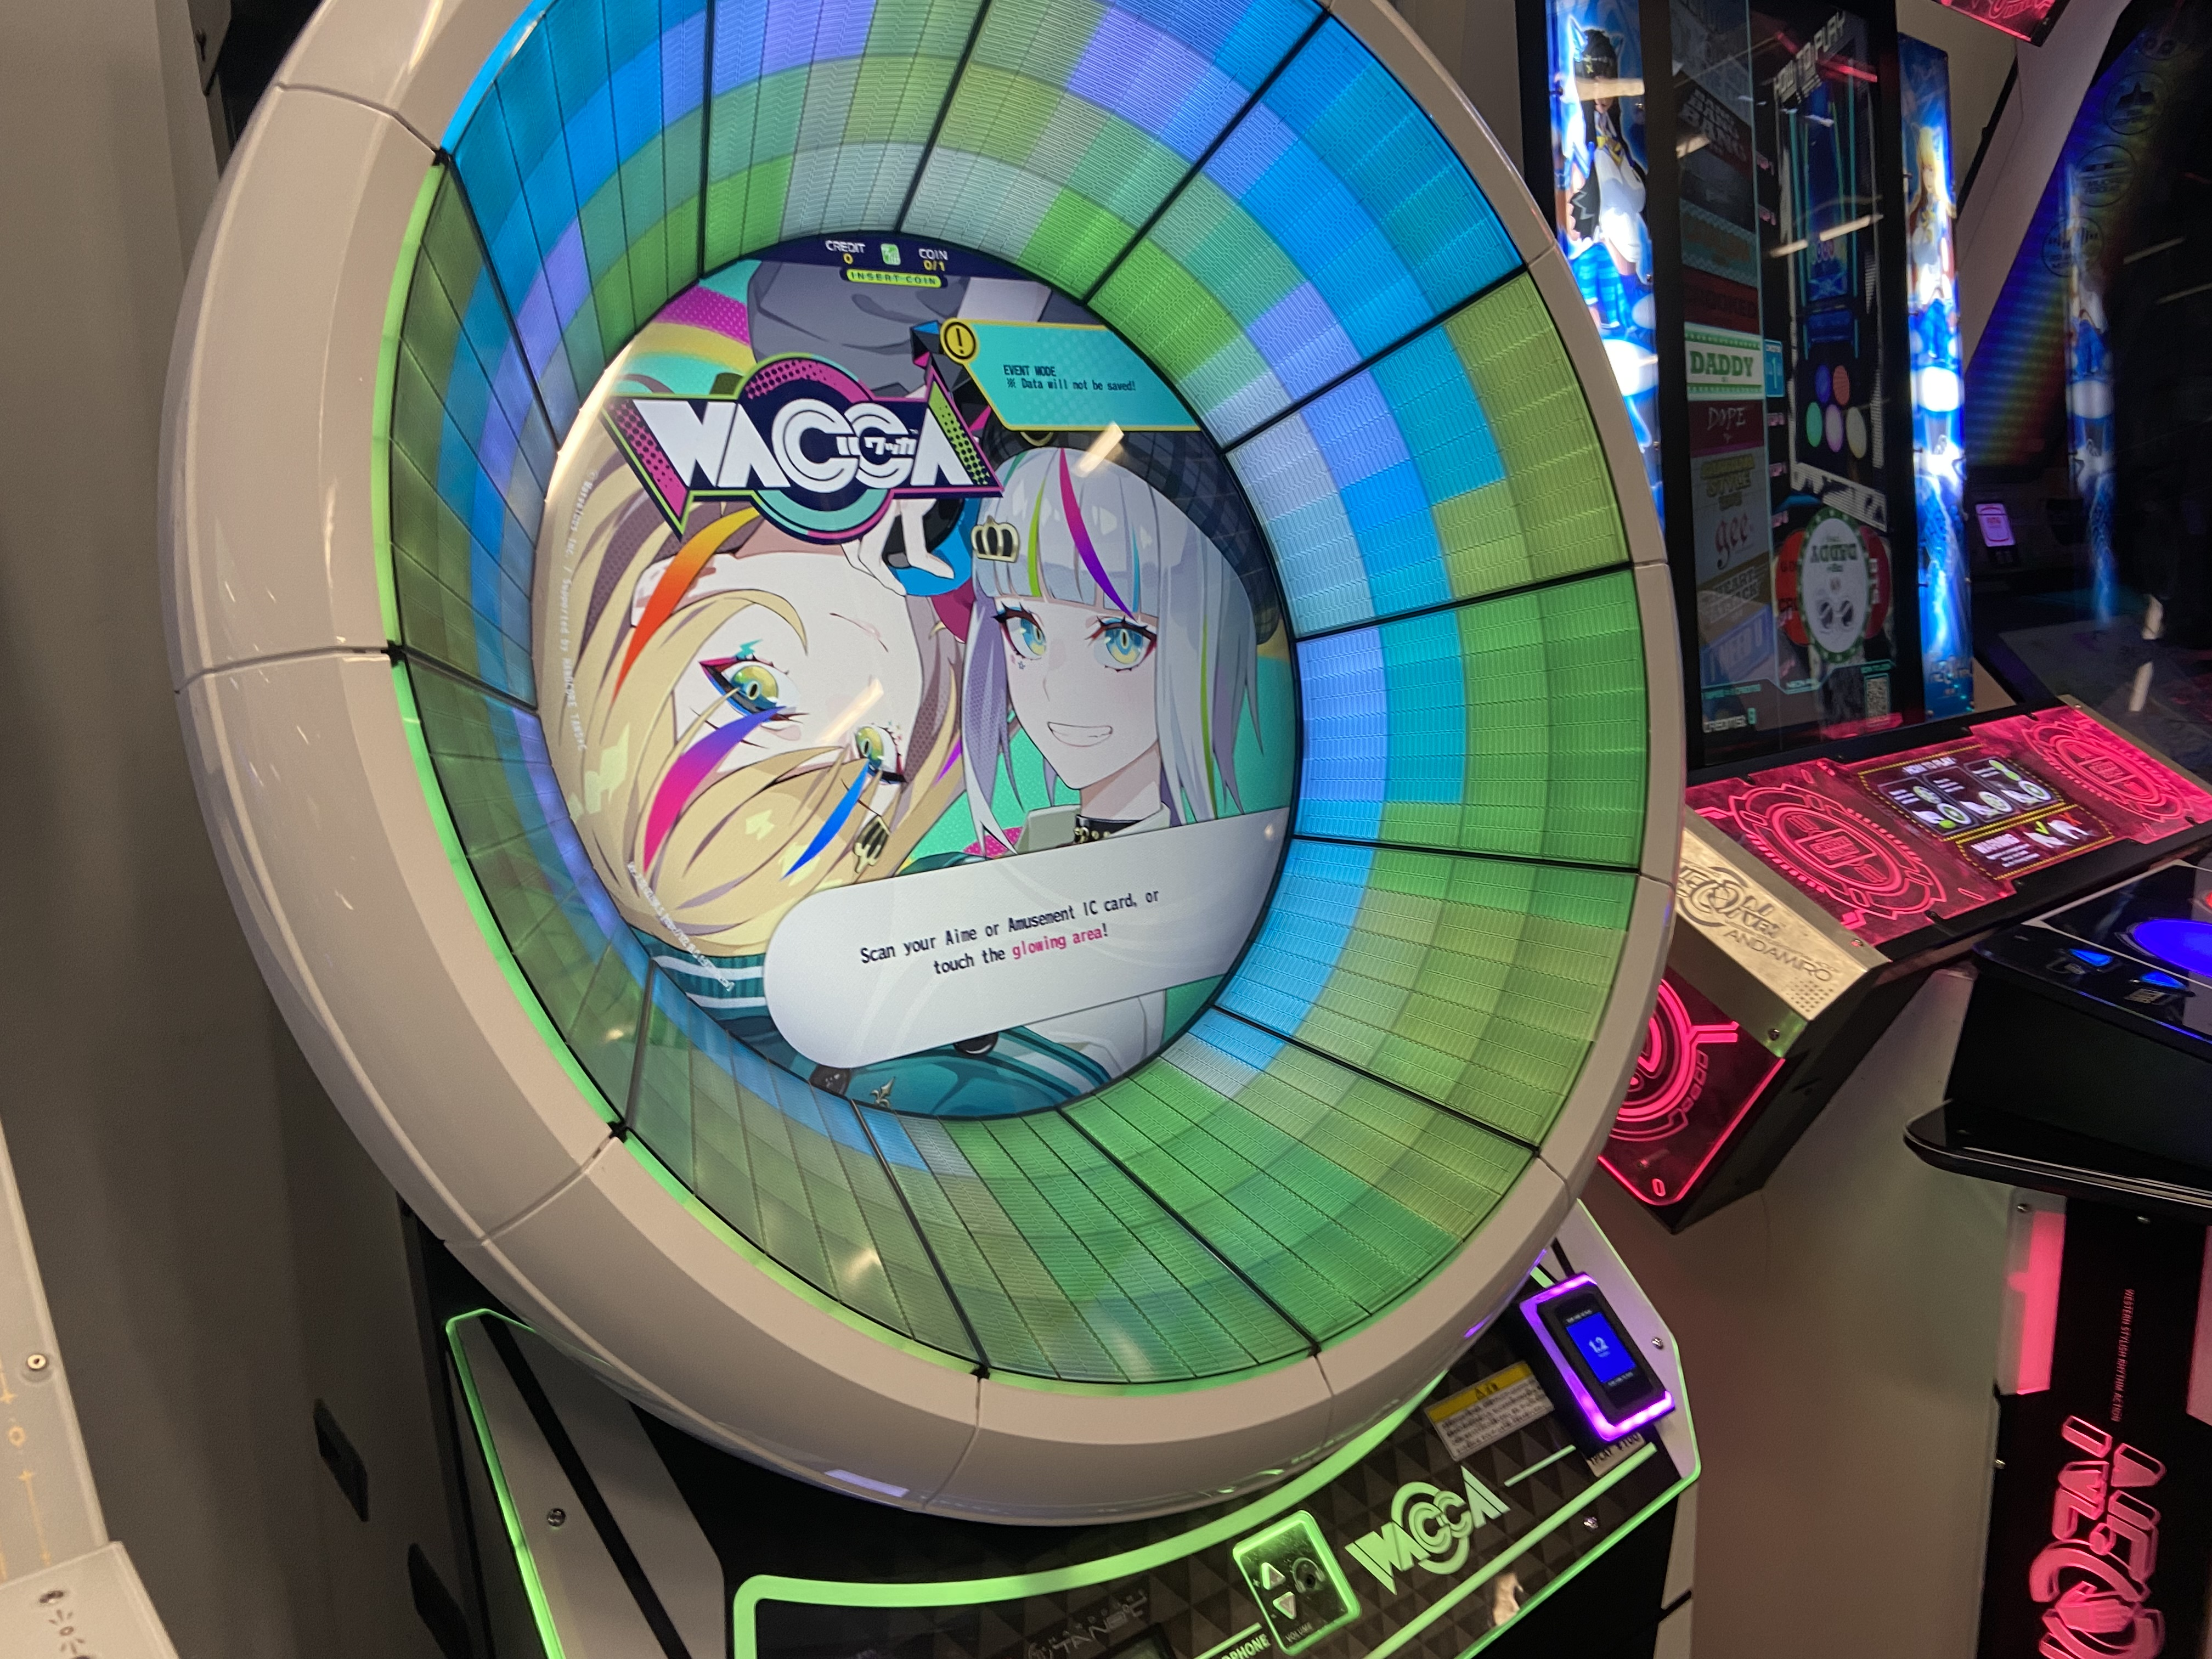
\includegraphics[scale=0.1]{obrazki/waccaarcade.jpg}
    \caption{\textit{WACCA} arcade booth, showing its unique form and controls. \cite{waccaarcade}}
    \label{fig:wacca_arcade}
\end{figure}

The genre of rhythm games also has immense value as an educational tool, as shown through the release of \textit{Rocksmith} by Ubisoft. Instead of using a fake plastic controller, the game allows the player to plug in any real electronic guitar, making it the centerpiece of the game. The game’s interface is similar to \textit{Guitar Hero}’s stage, but approaching notes are more specific in order to instruct the player about what grips and strings are supposed to be used. Due to using a real guitar instead of a plastic device, the game was received as a great development milestone in the genre, highlighted by the educational value provided by playing on an actual instrument, as creating a digital rhythm game with real instruments as an input device was a notable achievement for the genre. The game is developed to this day in the form of \textit{Rocksmith+} -- a free-to-play title available on PC, monetized through in-app purchases of songs and lessons.

As Fares Kayali stated in his thesis \textit{Playing Music: Design, Theory, and Practice of Music-based Games} \cite{faresplayingmusic}:
\begin{quote}
    Overall, rhythm games have changed very little over time. The only changes Harmonix made to the much older Konami games concerned perspective and direct control of the underlying soundtrack. Distinction between rhythm games revolves mostly around the different input devices. From floor mats in DDR, to turntables or guitars, a variety of interfaces have found their way into the homes of rhythm game fans (Kayali 2008: 48).
\end{quote}
Notably, despite the fact that all rhythm games have similar core gameplay, with the development of technology this genre has been able to expand the player experience through the use of new input devices and unique approaches to gameplay. With the rise of technologies such as virtual reality or touch screens, rhythm game developers have utilized new solutions to create new experiences. Because of this, the creativity of game designers is no longer limited as it was in the past.

\section{Immersion in rhythm games}
In order to immerse the player in the game, previously described core gameplay mechanics are further enhanced by visual, auditory and tactile feedback. This is done by using additional hitsounds, visual effects, or in the case of arcade cabinets, through decorations around the cab. As a result, it is easier for the player to get into the flow state -- a state of mind where the player is fully immersed in the game and is able to perform at their best. Additionally, in that state the player obtains the most enjoyment from the performed activity. As Jenova Chen says in his MFA thesis \cite{chen2006flow}:
\begin{quote}
    People associate many feelings with ``fun'': the sense of timelessness, of being at one, of exhilaration, focus, immediacy. (...) There is universal agreement that without a dynamic balance between the challenge of an activity and the ability to meet that challenge, fun is something we are definitely not having. Interestingly, making it possible for anyone to find exactly the right amount of challenge to engage with the exact abilities is the only way to access Flow. This means that when work is fun we have created complex, but negotiable challenges, challenges that allow the individual to engage or disengage, to work harder or work safer. [Dekoven DeepFun.com] At this point, fun can be defined as Flow, a balance of the relationship between challenge and ability (Chen 2006: 7).
\end{quote}
As the player can adjust the desired difficulty level, it is easy to find the perfect balance between the challenge and player’s ability to meet it. This is the reason why rhythm games are accessible for both beginners and advanced players, who are familiar with the genre already. In both cases, the gameplay and game design provide good conditions for the player to get into the flow state. No matter the skill of the player, elements of the gameplay, UI and auditory feedback play a crucial part in the immersion and entering the flow state. Described feedback is especially visible in \textit{Beat Saber} -- a Virtual Reality rhythm game, where the player is fully transferred into the game world through VR headset and controllers. The gameplay of \textit{Beat Saber} tracks the movement of the player’s body and controllers which are held in both hands, requiring the player to slice approaching notes with two swords (controllers) and avoid obstacles by actually moving their body. Upon slicing the notes, the game provides auditory, haptic (using the vibration of controllers) and visual feedback -- the sight and sound of the note being cut in half inform that the note had been correctly cut, providing the instant response matching the rhythm of the currently played song. While being surrounded by the game world in VR, the score and combo counter is shown to the player during the gameplay, making it possible to keep track of the performance during gameplay. As every other rhythm game, the player can start by playing easy levels and understand the basic mechanics of the game, grasping its rules through the observation of the outcome and instant feedback. The game’s UI is intuitive -- for example, the notes which are approaching the player have an arrow which indicates the required direction of the slice. If this mechanic is too difficult for beginners, it is possible to turn on the no-fail mode or make the notes possible to slice from all directions. This way, the game is accessible for the most novice players who also need to get used to VR and controllers.

\begin{figure}[h]
    \centering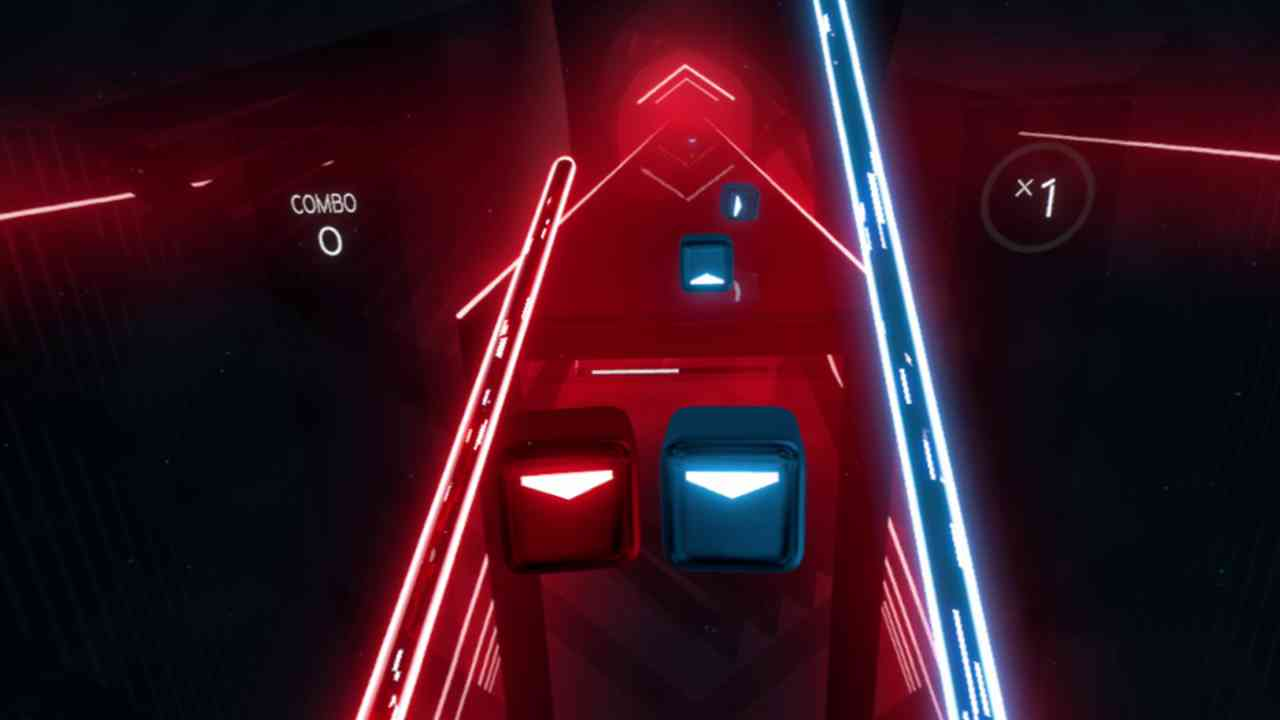
\includegraphics[scale=0.3]{obrazki/beatsaber.jpg}
    \caption{\textit{Beat Saber} -- screenshot of the gameplay. The red notes are corresponding to the sword held in the left hand, and the blue ones which correspond to the sword held in the right hand. The arrows placed on the notes are indicating the direction of slicing. \cite{beatsaber}}
    \label{fig:beatsaber}
\end{figure}

Fares Kayali emphasizes this aspect of immersion in his thesis \cite{faresplayingmusic}:
\begin{quote}
    When designing a game, one must focus on the experience of the player and his or her involvement with the game. Ideally, an immersive game experience suspends the player in a state of flow. Being immersed and acting in flow with a game world leads the player to a ``willing suspension of disbelief'', a mental state first described by Samuel Taylor Coleridge (1817) in relation to literature and the reader. It signifies the willingness of the reader (or in this case the player) to ``buy into'' the prepared fictional world, putting aside rational doubts about its authenticity. The recipient suspends disbelief, diving into the presented world and greatly raising involvement. To enhance this state of immersion, a fictional world must provide a consistent setting that does not disrupt this willing suspension of disbelief (Kayali 2008: 112).
\end{quote}
Through immersing the player fully into the game world by the Virtual Reality, the experience of \textit{Beat Saber} is more likely to put these rational doubts of the player aside, enhancing the player’s focus and commitment to the gameplay. Moreover, the \textit{Beat Saber}’s feedback is satisfying and rewarding, making the world presented in Virtual Reality more consistent with the musical experience.

Another example of such usage of feedback is \textit{SOUND VOLTEX} -- an arcade rhythm game developed and published by BEMANI, featuring a unique controller with four main buttons placed in the middle, two wide buttons placed below main buttons and two knobs placed on the sides of the controller.

\begin{figure}[h]
    \centering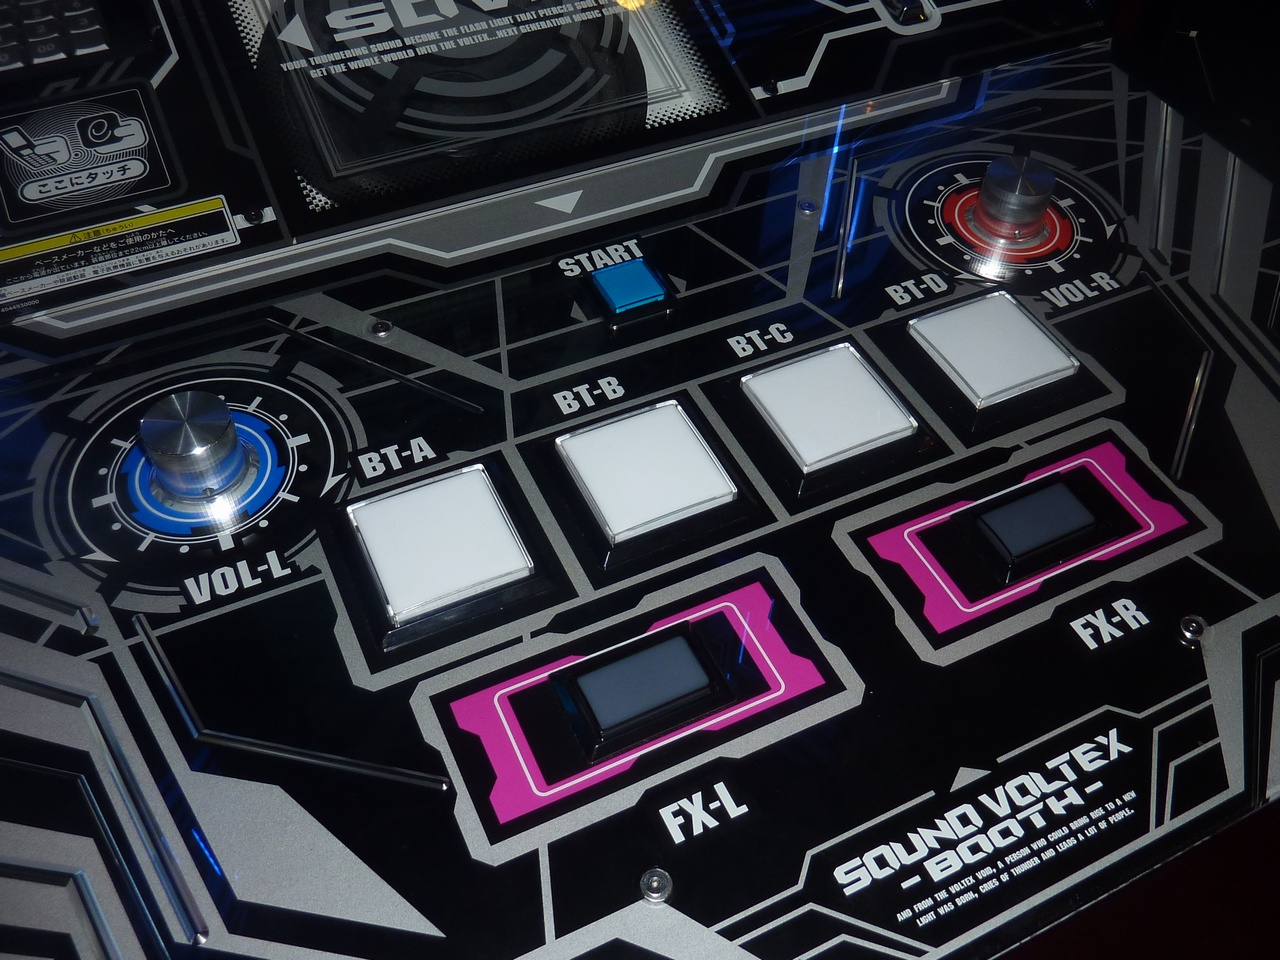
\includegraphics[scale=0.75]{obrazki/sdvxcontroller.jpeg}
    \caption{\textit{SOUND VOLTEX} Controller -- the composition of its controller makes it stand out from other rhythm games cabinets.\cite{sdvxcontroller}}
    \label{fig:sdvx}
\end{figure}

Once the player has chosen a track from the list and the difficulty of the chart (song), the game is played on a vertically scrolling road with 6 segments with aforementioned notes that correspond to the physical buttons. The gameplay consists of 3 types of notes: Basic white notes that appear in the middle 4 segments, corresponding to the white buttons; Orange notes which appear beneath white notes and cover 2 middle segments -- corresponding to the wide buttons placed on the bottom of the controller; Two lasers marked with vivid colors: Blue (left knob) and pink (right knob) that appear on the outer segments of the road. In order to better understand the game and distinguish types of notes, the buttons on the controller are signed with names: knobs are named VOL-L (left) and VOL-R (right), names BT-A, BT-B, BT-C, BT-D for white main ones, and FX-L and FX-R names for bottom, wide buttons. Thanks to the arrangement of the controller’s buttons and vivid colors of notes showed during the gameplay, the player can easily get used to reading the chart and hitting the corresponding buttons. As the note reaches the judgement line (above the representation of the controller), the player can see the accuracy of the hit -- the note is judged as CRITICAL, NEAR or MISS. The game also features a lifebar, which goes up as the notes are hit to the rhythm, or decreases if missed. In order to pass the chart the player must exceed the particular level of health bar (which differ from one difficulty to another). If the player is missing too many notes, it causes the song to CRASH, ending the course. Moreover, the buttons of \textit{SOUND VOLTEX} controller are satisfying to use, as they light up and give a firm, tactile response with a satisfying ``click'' upon pressing. On top of that, the modern design of the game’s cabinet and controller matches the futuristic aesthetic of the game, presented in the game’s gameplay, UI, illustrations and featured music, which includes many genres but revolves mostly around electronic genres. The game’s menu features characters in anime-style illustrations, with sci-fi inspired outfits, accessories and hairstyles, matching the futuristic aspects of the game. 

\begin{figure}[h]
    \centering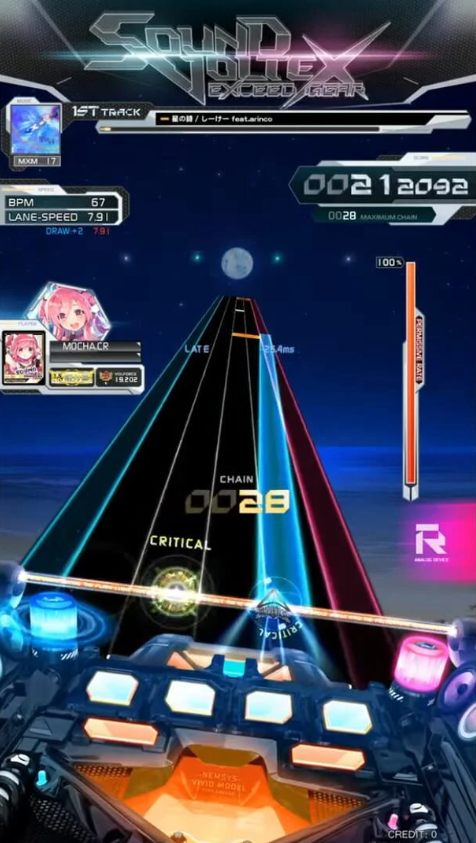
\includegraphics[scale=0.6]{obrazki/sdvx.png}
    \caption{\textit{SOUND VOLTEX} -- screenshot of the gameplay. The player is required to press the buttons and turn the knobs in the rhythm of the song. In this screenshot, the one can see the blue laser note which requires the player to turn the knob from left to right, which is further followed up by pressing up the orange note and then the white one. \cite{sdvx}}
    \label{fig:sdvx2}
\end{figure}

The auditory feedback of \textit{SOUND VOLTEX} is especially important regarding the immersion of the game. Similarly to \textit{beatmania}, \textit{SOUND VOLTEX} introduces audio effects upon every input made by the player through the controller. Every hit of the note and following the laser notes are mixing the original version of the song played, providing new experience from listening to it. As one song usually have few difficulties to play, the same song can have several remixes based on the density of notes to hit. The laser notes are making this experience even more immersive, as the ``laser'' sound produced by turning the knob is different depending on the direction of the turn and the speed rate. It comes along with the visual feedback of the game, as the whole stage is rotating accordingly to the knobs input. Such aspect is heightened when clearing sharp turns, in which the laser line crosses the road horizontally -- such laser notes require the player to turn the knob quickly, producing intense swishing sound effect that comes along with whole 360 degree spin of the scene. On the other hand, long orange notes that requires the player to hold the wide buttons are used to produce a sound effect that resembles a DJ turntable scratch. During the gameplay, the stage also zooms in or out to enhance the particular moments of the song -- such as more melodic or build-up parts with many notes to hit. It enhances the player’s experience and makes the chart easier to read, as zooming out shows more of the upcoming notes. Adding the haptic feedback which is produced by the controller’s buttons, the player can feel as they are actually performing and remixing the currently playing song. As Ian Bogost points out in his book \textit{How to do things with videogames} \cite{bogostmusic}: "Guitar Hero–style games offer a new perspective on musical performance by simulating the actual performance of music in an abstract but relatively direct way" (Bogost, 2011: 34). The author also implies that rhythm games can deepen the understanding of music throughout the play, highlighting that the performative aspect of rhythm games is a crucial part of the experience. Just as in \textit{Guitar Hero}, \textit{SOUND VOLTEX} allows the player to feel the music differently, as the player is not only listening to the song but also performing it.

Such connection of the visual, auditory and haptic feedback, plays a crucial part in immersing the player and evoking the flow state. As the feedback makes the gameplay more satisfying and enhances the rhythm, it is more likely for the player to enter the flow state, while enjoying the game to the fullest. Such experience provides better environment to focus on the play, as the full immersion makes the game easier to learn and master by players.

As Mihaly Csikszentmihalyi says in his book \textit{Flow: The Psychology of Optimal Experience} \cite{csikszentmihalyi1990flow}:
\begin{quote}
    As our studies have suggested, the phenomenology of enjoyment has eight major components. (...) First, the experience usually occurs when we confront tasks we have a chance of completing. Second, we must be able to concentrate on what we are doing. Third and fourth, the concentration is usually possible because the task undertaken has clear goals and provides immediate feedback. Fifth, one acts with a deep but effortless involvement that removes from awareness the worries and frustrations of everyday life. Sixth, enjoyable experiences allow people to exercise a sense of control over their actions. Seventh, concern for the self disappears, yet paradoxically the sense of self emerges stronger after the flow experience is over. Finally, the sense of the duration of time is altered; hours pass by in minutes, and minutes can stretch out to seem like hours. The combination of all these elements causes a sense of deep enjoyment that is so rewarding people feel that expending a great deal of energy is worthwhile simply to be able to feel it (Csikszentmihalyi 1990: 57).
\end{quote}

Analyzing aforementioned \textit{SOUND VOLTEX} mechanics and feedback regarding this quote, it is easy to observe how the game evokes the flow state. The provided satisfaction from the play is ensured by engaging the player in the task that may be completed in deep focus state -- starting from the ability to choose favorite song and the desired difficulty, followed by the instant feedback and responsible mechanics during the gameplay, ending the course with results, score and the feeling of accomplishment. Such design of the player’s experience provides a great environment that enhances the player’s engagement, supporting the ability to learn and master the game. Taking all of the described elements into the account, it is clear that elements that enhance the immersion are concomitantly evoking the flow state. As Steve Swink points out in his book \textit{Game Feel: A Game Designer’s Guide to Virtual Sensation} \cite{gamefeel}: "When players refer to being immersed in the game, part of what they’re experiencing is flow" (Swink 2009: 23). It is important to note that immersion and flow are two different things, but they are closely related.

\section{The importance of flow in rhythm games}
In order to evoke flow state in the player, the game must be designed in such a way that the task and its environment enhance immersion and engagement. As rhythm games differ from other game genres that include narratives, plot, quests and objectives, it may seem that flow state can be applied differently in this genre. However, the core elements of flow state are objectively the same as in any other game or activity.
Firstly, it is crucial to understand the fundamentals of flow state and its importance in the context of video games. As Jenova Chen describes in his MFA thesis \cite{chen2006flow}, Mihaly Csikszentmihaly distinguishes eight component that are required to achieve the flow state:
\begin{quote}
According to Mihaly Csikszentmihalyi’s well-documented research and wide-scale
gathering of personal observations, the phenomenology of Flow has eight major
components.
\begin {itemize}
\item A challenge activity that requires skills
\item The merging of action and awareness
\item Clear goals
\item Direct feedback
\item Concentration on the task at hand
\item The sense of control
\item The loss of self-consciousness
\item The transformation of time
\end {itemize}
Not all of these components are needed for flow to be experienced. [Csikszentmihalyi 1990](Chen 2006: 7).
\end{quote}

These components are crucial to evoke flow state throughout various activities, including video games. Regarding games, there are three core elements that Jenova Chen identifies:
\begin{quote}
\begin {itemize}
\item As a premise, the game is intrinsically rewarding, and the player is up to play the game.
\item The game offers right amount of challenges to match with the player’s ability, which allows him/her to delve deeply into the game.
\item The player needs to feel a sense of personal control over the game activity. 
\end {itemize}
As a result, the game will make player lose track of time and self-consciousness. (Chen 2006: 7)
\end{quote}

Regarding rhythm games, such criteria are meet through merging the game’s mechanics with music. As mentioned in the curator’s note of ``A MAZE. Interact'' \cite{MAZE} catalogue: ``Music games exemplify the generally ambivalent nature of rules: whilst restricting action space, they produce new opportunities for interacting with music.'' (Liebe and Wiedemann 2010: 5). Performing the task is rewarding in itself, as the player can feel the satisfaction of hitting the notes to the rhythm of the music instantly, no matter the difficulty. As the player becomes more skilled at the game, they can unlock and play more difficult levels, always adjusting the game’s difficulty to their current skill level. Following the definition of flow state, the balance between skill and challenge plays fundamental role in maintaining the flow state. If the task difficulty is too high, the player is unable to enter flow state, as the task is evoking anxiety. On the other hand, if the capabilities of the player exceed the challenge, the player will become bored. The safe space between anxiety and boredom is determined as \textit{flow zone}.

\begin{figure}[h]
    \centering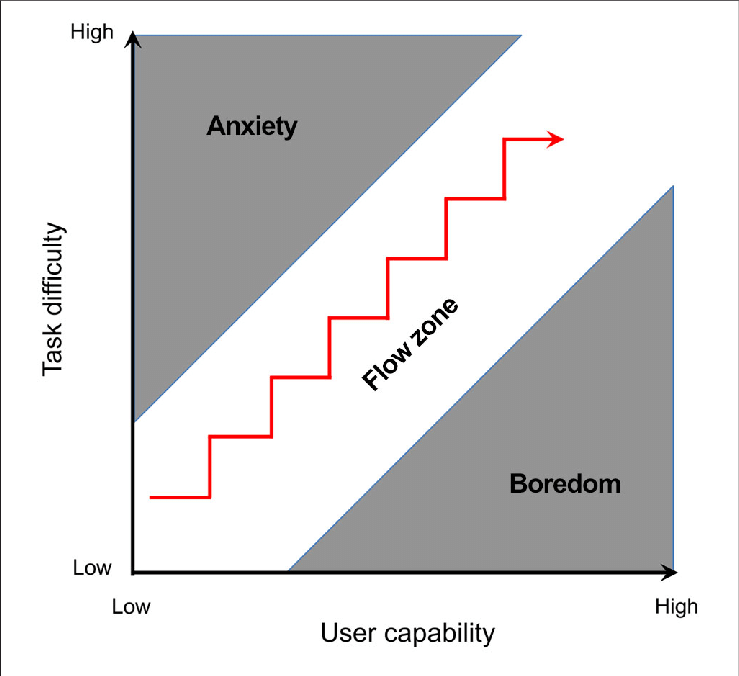
\includegraphics[scale=0.3]{obrazki/flowstategraph.png}
    \caption{\textit{Csikszentmihalyi’s flow state} -- graph showing how does the balance between the player’s skill and the game’s challenge influence the flow state.
    \cite{csikszentmihalyi1990flow}}
    \label{fig:flowstategraph}
\end{figure}

In rhythm games, as the player can always pick the desired difficulty level, it is easy for the player to maintain the flow state. If there is a difficulty that was too hard in the past, the player can always come back to it later, when they feel more confident with their capabilities. This replayability also allows the player to improve their previous scores, which can be a source of motivation to keep playing the game. Consequently, rhythm games meet the criteria for both casual and hardcore gaming, as Jesper Juul describes in his book: \textit{A Casual Revolution: Reinventing Video Games and Their Players}\cite{casualrevolution}:
\begin{quote}
    In other words, these games are very different depending on what players are trying to achieve. For players who want to relax playing a song they like, the games fulfill the role of casual games where even an imperfect performance of a song on an easy level of difficulty can be a satisfying experience. However, for players who want to master the games or win a competition, the games’ punishment structures match traditional hardcore design. In this case, the player must keep replaying a given song in order to perfect his or her skills (Juul 2010: 129).
\end{quote}

Interestingly, an article \textit{Predicting Chart Difficulty in Rhythm Games Through Classification Using Chart Pattern Derived Attributes}, included in book \textit{Computational Science and Technology}, highlights the issue of predicting the difficulty of a song charts in rhythm games: 
\begin{quote}
    An issue that exists, not just in \textit{Dance Dance Revolution}, but in rhythm games in general is the estimation of a chart’s difficulty level. While many methods and studies exist in generating and predicting chart attributes, there is no clear methodology existing in determining the optimal difficulty of a given chart (Caronongan and Marcos 2021: 193).
\end{quote}
 
The importance of setting the right difficulty for a given chart is undeniable, as it nurtures the player and informs them about their current skill level. What is more, it is important to create a wide variety of difficulty levels, in order to allow the player to progress and polish their skills gradually. The authors of this chapter are pointing out that in \textit{Dance Dance Revolution}, the skill gap between charts' difficulties is too big -- "Some of the players, especially average players, are not satisfied enough with the charts because the charts in the appropriate difficulty level for the player are not prepared" (Caronongan and Marcos 2021: 194). This is a crucial aspect of the game design, as the player will not able to enter the flow state if the difficulty is too high or too low. As the authors of this article point out, the game should be designed in such a way that the player can gradually improve their skills and polish their performance. This is especially important for rhythm games, as they are often played in a competitive environment, where players are trying to achieve the best score possible. If the game does not provide a clear path for improvement, players may become frustrated and lose interest in the game.

Beside maintaining the flow state, games must also be entertaining when players enter the flow zone. As rhythm games revolve around music, it can be naturally achieved through the inclusion of music, which in itself is a source of entertainment. As usual, music is constructed in such a way that it catches the attention of the listener through its structure. The six primary parts of the song can correspond to the gameplay. As the song starts with intro, which is usually slower, the player can familiarize themselves with the rhythm and warm-up. As the song progresses and becomes more energetic, the player can expect more intense parts, that can be reflected in the gameplay. Such build-up prepares the player for the climax of the song, which is usually the most difficult part to play during a selected level. Typically, songs have slower parts between the intense chorus, in which the player can relax and prepare for the next intense part. After another intense part, the song usually ends with a slower outro, in which the player can relax with less difficult patterns of notes. As such structure is repeated in most songs, no matter the genre, even the most novice players can quickly understand that their play will resemble the structure of music that they listen to. This feeling of familiarity can reduce the potential anxiety when trying new difficulties, therefore enhance the entertainment coming from the play. This practice may resemble a process of learning an instrument, as mentioned in \textit{A Casual Revolution: Reinventing Video Games and Their Players}\cite{casualrevolution}:
\begin{quote}
    On some level it is true that these are not real instruments, but what makes them not real? The basic experience of playing these games is that if you do not press the buttons correctly there is no music, but if you press the buttons correctly, music appears—it feels as if you are making music. Interestingly, this is quite similar to learning to play an instrument (...) (Juul 2010: 115).
\end{quote}

Because of this natural familiarity, creating a songlist that is fun to play could be more intuitive than it may seem. As Fares Kayali describes in \textit{Playing music: design, theory, and practice of music-based games} \cite{faresplayingmusic}: 

\begin{quote}
    ``Since music is not completely graspable by a specific methodology, the process of formalizing music for music-based game design also depends upon its more abstract attributes. Kungel’s (2004) distinct audio parameters for movies includes dynamics, harmony, sound, melody, pause, rhythm, beat, and tempo. It provides game designers a list of parameters that can be accessed through player interaction or be changed as feedback to players.'' (Fares 2008: 60).
\end{quote}

With this insight in mind, game designers can choose songs for their game basing their choices on what they believe will resonate with the target audience. The music must match the game’s mechanics and control device, which in most cases will fit a wide range of music genres. Knowing that music is entertaining to listen to on its own, its ability to enhance the player’s experience and support a flow state is primarily dependent on how well the level design is integrated with the featured music. The audio parameters described by Kungel’s should serve as a guide for game designers and as a reference for the level design and note patterns included in the song charts.

\section{Components of Flow in rhythm games}
Coming to the aspects of clear goals, the objective of playing a rhythm game can initially seem as simple as just playing the song. However, games without the imposed narrative are giving the player more freedom to set their own goals. As mentioned before, the player may choose, if they want to, play casually or hardcore. Since there are plenty of various rhythm games, players can also choose which game appeal to them the most. As highlighted by Juul: ``Games without goals or with optional goals are more \textit{flexible}: they accommodate more playing styles and player types, in effect letting you choose what kind of game you want to play'' (Juul, 2010: 138). This flexibility enables the player to naturally establish personal objectives. Liberating the player from the pressure of meeting the imposed goals makes more space for the player to actually enjoy the game and polish their skills at the same time. On the other hand, some rhythm games offer storymodes or quests that unlock new songs or levels after completion. While this may motivate the majority of players to keep playing, it also may be frustrating for those who want to have the freedom of choice right away.
As described, the approach to progression in rhythm games varies widely - from completely lacking the storymode or structured campaign, through incorporating optional mission-based elements, to featuring full storylines that must be completed in order to unlock the full content of the game. Taking these three levels as an example, this variety of imposed objectives and progression path can be observed across different rhythm games.
Games like \textit{osu!} or \textit{StepMania} do not have any story mode or campaign, as their content is centered around the content created by the community and online leaderboards. These games lack the predefined progression system, as all of the content is available through downloading the content created by the community. Apart from being a player, users can also become creators of the content, as they can create their own levels, skins or even songs. One interesting example of a collaboration between game developers and music creators is \textit{osu!}, since the game allowed to create and upload \textit{beatmaps} for any .mp3 file chosen by the \textit{beatmapper} (the user which creates the map for this particular game). This aspect was highlighted by Fares Kayali in \textit{Playing music: design, theory, and practice of music-based games} \cite{faresplayingmusic}: ``Through increasing possibilities for downloadable content, music-based games also act as distribution platforms for music.'' (Kayali 2008: 53). This solution raised questions about licensing music, as the original musicians were not asked if they want their songs to be used in the game - noteworthy, the game is constructed in such a way that the .mp3 file with the full song is included in the beatmap folder. For this reason, some beatmaps were removed by musicians who found out about it and were not quite happy about it \cite{osucontroversy}. Under pressure from allegations of using unlicensed music in the game and generating profit from it, the developer of \textit{osu!} -- peppy -- began to collaborate with musicians through the ``featured artists'' program, officially licensing songs from artists that were interested in being featured. 
However, beatmappers are still allowed to use any .mp3 file from their computer, so making the risk of distributing pirated music is not completely eliminated. Nevertheless, this solution created unlimited opportunities for players and content creators to gamify any music possible, at the same time promoting musicians, as many players can be introduced to their music throughout the game. This solution has its benefits and drawbacks, but leaving aside the moral part, this level of freedom in creative work has an impact on player and community engagement. It completely replaces the narrative aspect of the game, directing the player’s attention to content created by the community and the competition with other players. The game’s content is created in such a way that there’s always something new to play, encouraging the players to compete for the best scores on newest songs.

\begin{figure}[h]
    \centering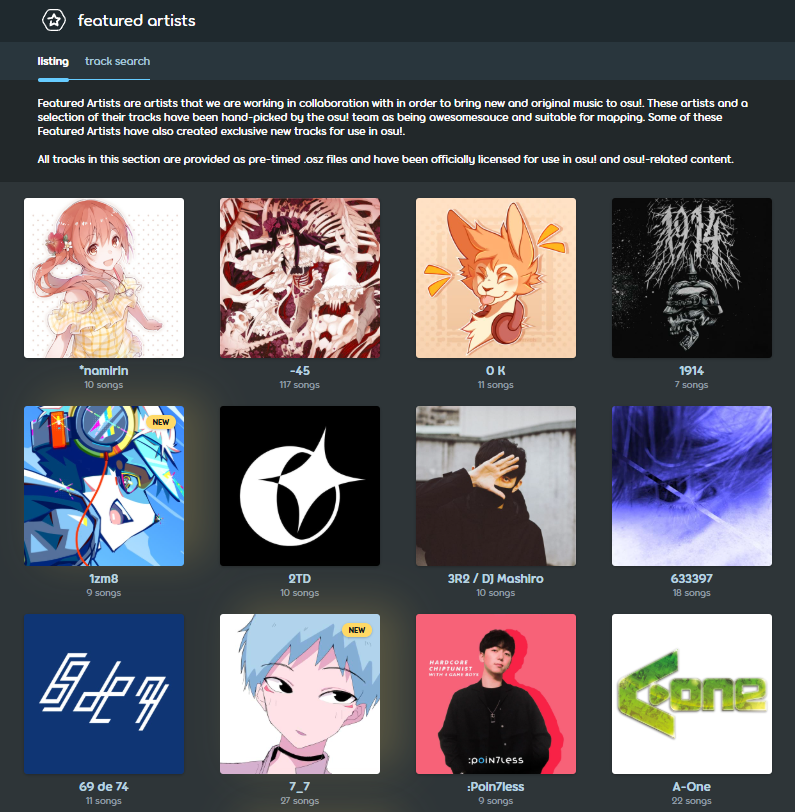
\includegraphics[scale=0.4]{obrazki/featuredartists.png}
    \caption{\textit{osu!} featured artists -- the program that allows the musicians to collaborate with \textit{osu!} and its' content creators. \cite{osufeatured}}
    \label{fig:osufeatured}
\end{figure}

Especially during the official and community tournaments, players are always competing on the same beatmaps. A notable element of this is the fact that beside creating the composition and shape of the level, the \textit{beatmappers} are also responsible for choosing the background image and the visual effects (storyboards) of their map. Additionally, they may include custom hitsounds that further enhance the desired experience of playing their content. As one can observe, the example of \textit{osu!} shows that the engagement of the playerbase may not depend on the content created by the developers or the procedurality of storymodes. In this regard, the designed mechanics of the developers can simply serve as an instrument for the game community to create immersive content that evokes flow state. As players can create their own beatmaps with the music of their choice, the invocation of the flow state can be taken to the next level. For example, if a player notices that an old beatmap is poorly designed and missing important aspects, they can create their own version with adjustments. An important aspect of curating beatmaps for \textit{osu!} is that the beatmap needs to go under the procedure of testing and review in order to be qualified as a ranked map -- only then it can contribute to the personal scores of players and the global leaderboard. Since the map must be polished and meet certain requirements in order to be playable and ranked, the testers must also reassure that it will be entertaining to play -- therefore, the acquisition of Flow Zone during playing the beatmap will be assured by the curators and community feedback. 

On the contrary, the inclusion of a lightweight mission system is present in \textit{Groove Coaster: Wai Wai Party!!!!} for Nintendo Switch. The game offers missions and challenges that require a wide range of effort and time. Some of the missions require the player to play a certain song only once, while other challenges obligate the player to play every song of a given category and difficulty level. These challenges are devoid of any narrative, which in this case is rather a better solution, take less time and leave the player with clear and obvious goals. What may be frustrating for some players is fact that, these missions are included as a progression tree that requires completing one mission to progress to the next one. As a solution, the player obtains in-game currency throughout the play and may auto-complete desired missions by spending the currency.

\begin{figure}[h]
    \centering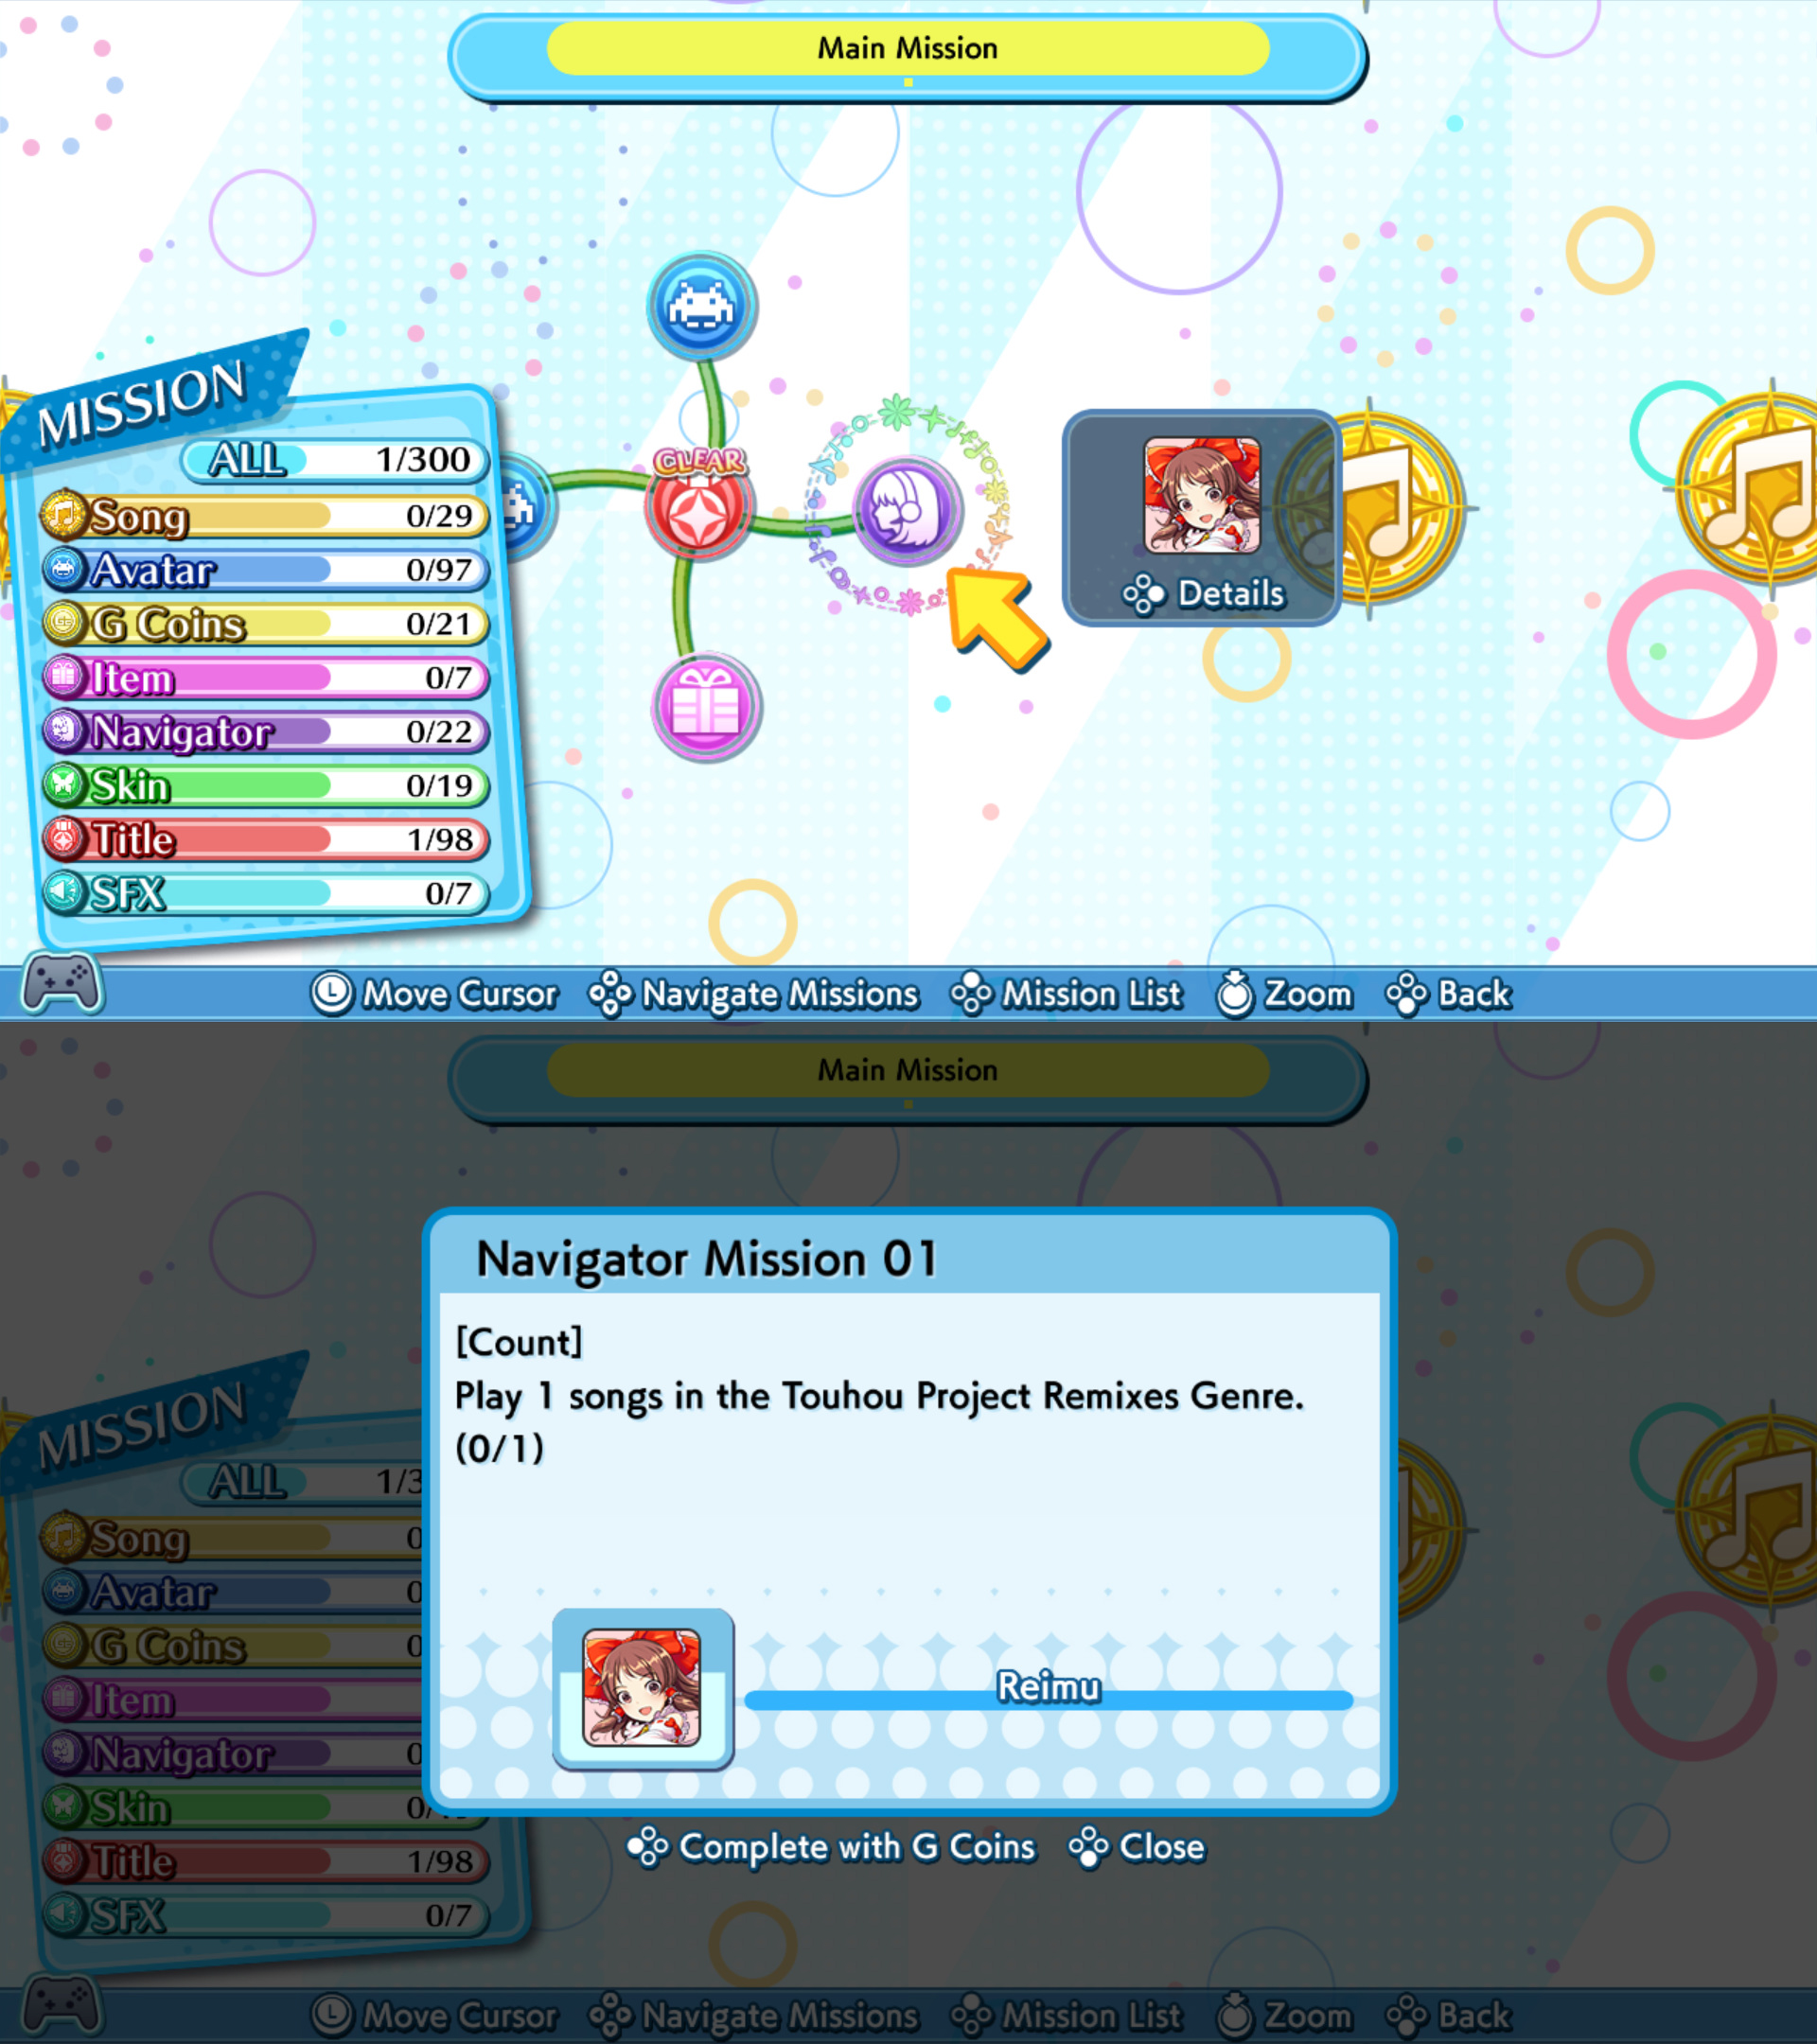
\includegraphics[scale=0.2]{obrazki/groovecoastermissions.jpg}
    \caption{Screenshot of the missions in . The player is required to complete the mission in order to progress to the next one. \cite{groovecoastermissions}}
    \label{fig:gcmission}
\end{figure}

Unlike \textit{osu!}, the content of \textit{Groove Coaster: Wai Wai Party!!!!} is procedurally designed by its developers, leaving the player base fully dependent on new updates and DLCs that are available with payment. This approach to the player experience is quite different from the aforementioned \textit{osu!}, as the game has limited catalogue of content that the player may unlock and play. Therefore, games with such approach can be fully completed by the player. This approach is more similar to other games that encourage the player to play in order to fully complete the game. Although the game is designed this way, the difficulty level and the skill needed to complete the hardest songs are so high that most players will likely never manage to fully clear all expert-level songs.

An example of a game that incorporates a developed story mode is \textit{Guitar Hero III: Legends of Rock} for home consoles and PCs. The game features a single player and Co-op Career Mode. In single player Career Mode, the game puts the player in a role of a rockband member with a goal of becoming a rockstar and growing the band to the heights of fame and popularity. It is structured as a linear series of 8 tiers, presenting a fictional venue where the player performs the gigs. Each tier contains 4 or 5 songs and requires the player to complete current set of songs -- the player must complete at least 3 or 4 songs of the setlist (depending of the currectly chosen difficulty) to unlock the last part of the tier: Encore and a Boss Battle, some tiers conclude with only one, while others involve both. Passing the last part results in the completion of a tier. 

\begin{figure}[h]
    \centering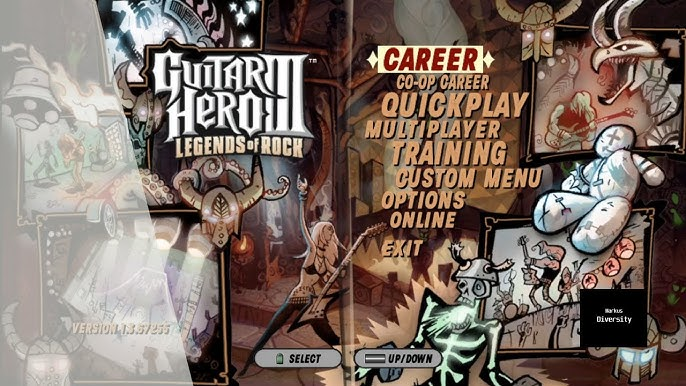
\includegraphics[scale=0.55]{obrazki/guitarherocareer.jpg}
    \caption{Screenshot of the \textit{Guitar Hero III: Legends of Rock} menu. The Career Mode is first on the list. \cite{careermodegh3}}
    \label{fig:ghero3}
\end{figure}

Progressing to other tiers further increase the difficulty of the songs. While passing through the songs, the player earns the in-game currency, which the player may spend in Shop in order to unlock new guitars, heroes and bonus songs. The Co-op career mode is similar to the singleplayer mode, but it features different setlist (songs) and lacks the unique Boss Battles. As observed, the Career Mode consists of three main, defined objectives: complete set numer of songs, defeat a boss or play an encore, progress to the next tier. Such structure provides clear goals for the player, thereby making the player immersed in the task at hand. The sequence of short-term missions helps the player to maintain focus and lead to long-term mastery, as the player is constantly improving their skills throughout the play. As the Career Mode starts with simpler songs and gradually introduce faster tempo and more complex patterns of notes, the aspect of increasing challenge ensures that the player will be enclosed in the Flow Zone, between the anxiety and boredom. Although the campaign is linear, the player has the ability to choose song order within setlist, providing the sense of control over the course. On top of that, the Career Mode includes elements that enhance the player’s immersion -- it portrays the player’s progression as an adventure of a rockband, which is additionally presented through the cartoon-like animated cutscenes and the visual design of the game. The game’s UI, artstyle and visuals further complement the experience of feeling like a member of a rockband, as the whole theme of the game revolves around rock music and the lifestyle of a rockstar. Obviously, as previously mentioned, the inclusion of real-life rock music which is present in every \textit{Guitar Hero} game, is a significant aspect of evoking the flow state -- in this case, the setlist of Career Mode also includes rock music created by real-life musicians. As Kayali Fares writes in \textit{Playing music: design, theory, and practice of music-based games} \cite{faresplayingmusic}: ``With Guitar Hero, Harmonix has successfully revived the vibe of rock’ n’ roll'' (Kayali 2008: 66).

The element of time transformation and the loss of self-consciousness are especially emphasized in arcade rhythm games. For practical reasons, arcade parks are often located in dark spaces, making the screens of arcade machines more visible. They are also tightly packed with machines, as renting more space can be costly. This dense arrangement of loud, flashy machines enhances the sensory-rich atmosphere. The unique environment, focused on games and entertainment, creates the illusion of being separated from the everyday world, making it easier to lose track of time. Arcade rhythm games, with their distinctive cabinets and controllers, stand out from other types of arcade machines. One of such arcade rhythm games is \textit{maimai} game series, developed by Sega and first released in 2012. The game includes both singleplayer and multiplayer mode, as its arcade machine consists of 2 player slots. The main display is a large circular touchscreen, surrounded by 8 buttons that are spaced evenly on the edges of the screen. In \textit{maimai}, the core gameplay revolves around responding to ring notes, which emerge from the center of the screen and travel outward toward the edge of the screen, aligning with one of the eight physical buttons arranged around the perimeter (judgement line). These are large, responsive pads that light up and provide tactile feedback, integral to the gameplay. Additionally, tap notes and slider notes appear on the touchscreen itself, requiring the player to tap or swipe on the screen with their hand. 
Similarly to other rhythm games, the player’s input produces in-game hit sounds and visual effects, creating a satisfying feedback loop that enhances immersion and flow state. As the game’s cab include two player slots, it encourages socialization with other players. The players can decide if they want to compete with each other in VS mode, or play along in Sync Mode -- in which the objective is to pursue the best score possible and synchronization, measured as a percentage. The game cab includes an IC card reader, on which the players can save their scores, unlock additional content and customize their personal profiles with currency obtained through achievements and events that include time-limited missions. Player profiles show not only best singleplayer scores, but also include Max Sync, which shows the highest combo (consecutive hit of notes without missing) achieved with the other player in Sync Mode.

\begin{figure}[h]
    \centering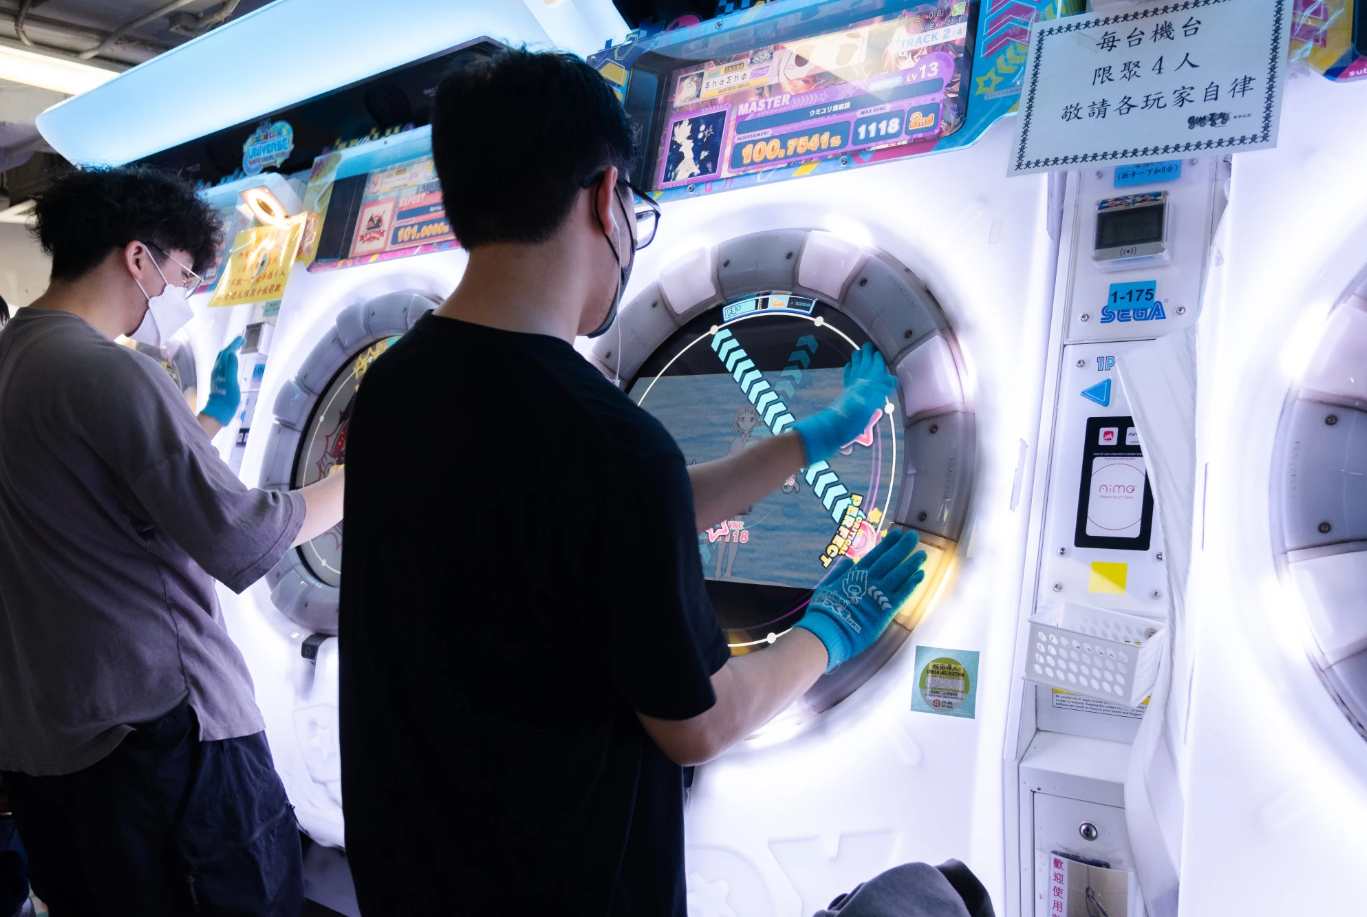
\includegraphics[scale=0.4]{obrazki/maimai2.png}
    \caption{The arcade cabinet of \textit{maimai DX} -- the players are playing the game together. The player on the left side clears the slider through sliding his hand across the touchscreen, while tapping a button with his other hand. Above the main screen there is a vertical display showing the player's profile and stats.\cite{maimai1}}
    \label{fig:maimaicabinet}
\end{figure}

Including such mechanics and in-game content that revolves around socializing with other players, the game encourages the players to play together and share their experience. Even while waiting in the queue for play, the players can talk to each other and watch the other players and cheer for them, which creates a sense of community. Combining this with the setting of arcade parks, the players can easily lose track of time and become fully immersed in the game and it’s environment. Taking into account the social aspect, the transformation of perceived time is further enhanced. This meaning of socializing during the play is described by Jesper Juul in \textit{A Casual Revolution: Reinventing Video Games and Their Players} \cite{casualrevolution}:
\begin{quote}
    Our pursuit of game goals makes the playing of games emotional even if we cannot point to any emotional content in the rules of a specific game. I think this can be
    extended to multiplayer games by thinking about how goals work in social contexts: players play for personal goals, are aware of the goals of other players, and the shared understanding of intentionality makes game actions socially meaningful (Juul 2008: 126).
\end{quote}
This aspect of socializing and sharing the experience with other players is crucial in evoking flow state, as it creates a sense of community and belonging. The players are not only focused on their own performance, but also on the performance of their friends or other players, which can enhance the overall experience. This aspect is especially important in arcade rhythm games, where the environment and the social aspect play a significant role in creating an immersive experience that evokes flow state.
